\documentclass{article}

\usepackage{hyperref}
\usepackage{parskip}
\usepackage{amsthm}
\usepackage{amsmath}
\usepackage{amssymb}
\usepackage{wrapfig}
\usepackage{graphicx}
\usepackage{listings}
\usepackage{color}
\usepackage{fullpage}
\newcommand{\code}{\texttt}

\author{Micah Wylde\\Jeffrey Ruberg}
\date{\today}
\title{Autonomous Agents:\\
A Hybrid Dynamical System for Vehicle Navigation\\
Comp 352}

\begin{document}
\maketitle

\section{Introduction}
Self-driving cars hold much promise for saving fuel, time and
lives. Human-driven vehicles are responsible for millions of traffic accidents
and over 30,000 deaths annually in the US alone. Humans can also make poor
decisions in regards to routes, leading to traffic jams and wasted fuel. Safe,
effective autonomous cars could largely solve these issues. AI researchers have
been interested in the potential for vehicular navigation since the 1960s. In
order to spur development in this area, the Defense Advanced Research Projects
Agency (DARPA) organized the Grand Challenge in 2004, which tasked contestants
to build cars which could autonomously navigate a 142 mile-long course in the
Mojave desert. Though none of the vehicles could finish the course, a second
competition the next year was more successful. Four teams finished in the
allotted time, traversing a treacherous 132 mile desert course with no human
guidance. Building on this achievement, in 2007 DARPA organized the Urban
Challenge which took place in a simulated suburban environment. To win, cars had
to navigate a maze of streets while accounting for other traffic and following
California traffic laws at all times. Six teams finished the 61 mile course with
the winner, ``Boss'' from CMU, taking a little more than four hours
\cite{robotic_cars}.

There are many challenges involved in autonomous driving and robot navigation in
general. In the real world one must deal with unreliable and imperfect sensor
data, imprecise localization technologies and other perception issues. Even in
simulation the challenges of successful navigation are immense. Cars must follow
traffic laws, get to their destination quickly and efficiently and act safely at
all times, even in unexpected situations. As far as the actual navigation, there
are two general approaches: deliberative and reactive. As an example of the
former, $A^*$ is an efficient and optimal graph search algorithm which is very
effective at finding the best route between two points but cannot handle the
dynamism of the real world. Dynamical systems-based navigation is a reactive
strategy that uses force fields to guide agents away from obstacles and towards
their target. However, it is purely local and has trouble finding optimal paths
to distant goals. In this paper we present simulated agents which use each
technique as well as a hybrid agent which makes use of $A^*$ for global
navigation and dynamical systems for local navigation.


\section{Autonomous Driving}

\subsection{Simulation}

\section{Methods}

To create an autonomous agent that navigates while simulating a car's behavior
and traffic laws, we took three general approaches: deliberative planning
through $A^*$ search, reactive navigation through a dynamical system, and a
hybrid of deliberative planning and reactive motion. The system architecture
consists of a server and a separate client for each agent.

\subsection{Simulation}
To provide a realistic environment for navigation tests, we used real-world map
data from OpenStreetMap.org, which provides XML-formatted maps for the entire
world. The data format, called OSM, provides a graph representation of a road
system where streets are represented by placing nodes wherever the road turns or
intersects other roads and edges connecting each node. To provide testing data,
we used the website to export maps of Hayward, CA and Santa Cruz, CA. We wrote a
program, osm\_convert, which converts an OSM XML file to a YAML\footnote{YAML (a
  recursive acronym for YAML Ain't Markup Language) is a language-independent
  data serialization standard which allows easy conversion of data structures to
  and from a string representation.}

In order to make a map suitable for driving, we generated \textit{roads} from
each edge by creating parallel lines from the edge a constant ROAD\_WIDTH apart.

\subsection{System Architecture}

The project is written in Ruby, specifically JRuby\footnote{JRuby is an
  implementation of the Ruby Programming Language on top of the Java Virtual
  Machine, which allows integration between Java and Ruby code} to utilize
Java2D for the graphical display. As a result, the server code runs solely under
JRuby, but client code can additionally be run using Ruby 1.9. Agents are
represented both on the client and server end; server agents perform motion and
display-related calculations, and client agents contain all the navigation
inference and decision-making and ultimately send decisions (restricted to
behavior variables) back to the server again.

\begin{figure}[h]
  \begin{center}
    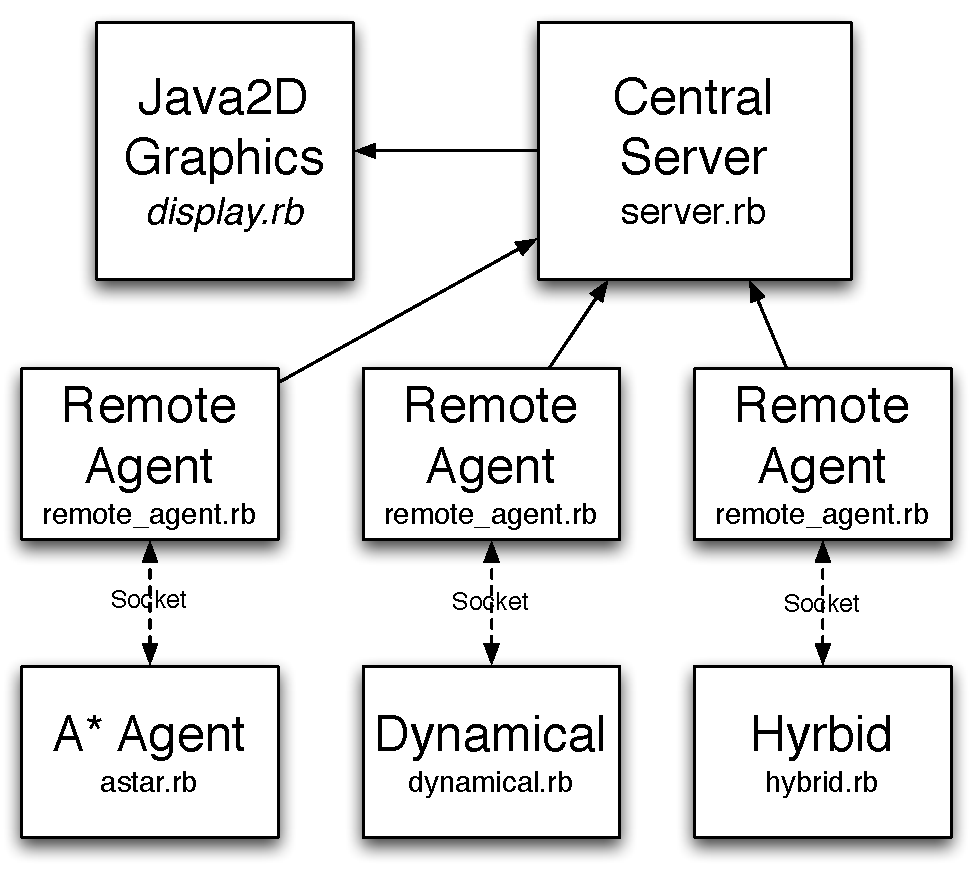
\includegraphics[width=0.5\textwidth]{architecture}
  \end{center}
  \caption{The system architecture of the simulation. Solid lines connect
    components included in the same process, while dotted lines indicated socket
    connections between discrete processes.}
  \label{architecture}
\end{figure}

A brief description of the various source files will follow.

\begin{description}
\item[app.rb] This file is the point of entry for the program. This same entry
  point is used to, based on various command-line options, start a server, start
  a new agent, or run tests.

\item[client\_agent.rb] This file contains the \code{ClientAgent} class, the
  super class which every client agent inherits. Client agents receive messages
  from remote server agents, process the message (based on their form of
  navigation), and then send back a response in their behavior variable space.

\item[constants.rb] This file contains various general constants that may be
  used in several locations or files, or that may be particularly useful to
  tweak with.

\item[display.rb] This file contains all of the display code used to generate
  our rendering of the world.

\item[map.rb] This file contains the classes, specifically \code{Map}, which
  encode information provided from real map data.

\item[pqueue.rb] A priority queue implementation useful for $A^*$ search.

\item[remote\_agent.rb] This file contains the \code{RemoteServerAgent} class,
  which is a subclass of \code{ServerAgent}. Essentially, a remote server agent
  is a server agent which is tied to a specific client agent and communicates
  with that client agent.

\item[server\_agnet.rb] This file contains the \code{ServerAgent} class, which
  contains all the base representation and calculations needed for an agent (for
  example, the server agent computes various points needed to display the agent
  graphically).

\item[server.rb] This file contains the socket server to which new agents
  connect.

\item[socket.rb] MICAH

\item[util.rb] This file contains a collection of geometry classes
  (\code{Point}, \code{Vector}, etc.) which are useful in the display and other
  various places (most notably in dynamical navigation calculations).

\item[agents/astar.rb] This file contains a client agent that deliberatively
  plans paths using $A^*$ search.

\item[agents/dynamical.rb] This file contains a client agent that navigates
  through a purely dynamical system-based approach.

\item[agents/hybrid.rb] This file contains a client agent that navigates through
  a combination of deliberative planning and dynamical systems.

\item[agents/simple.rb] This file contains a very primitive client agent (that
  can hardly be called an agent) which allowed us to easily test the motion
  calculations performed by server agents.

\end{description}

\subsection{Simulation Environment}

Our environment takes place in a graphical world we have constructed from
scratch. We start with real map data specifying nodes (intersections) and
connections (roads) between nodes, and create a graph representation; we also
convert positions specified in terms of latitude and longitude into a scale of
meters (where the minimum latitude position is given an x-coordinate of zero,
and likewise for longitude and y-coordinates). We mostly store the road data as
this graph of nodes and neighborhood relationships, but we also create road
objects which own wall line segments; while the map is being processed, we also
clip/extend these walls to create realistic-looking chunks of road between two
nodes.

To run the display, we start a server by running the script \code{bin/driving}
without any command line arguments (or with arguments to specify window geometry
or map file). In the display, we have implemented mouse dragging, zooming,
pausing, agent centering (on by default), and agent placement/manipulation.


\subsection{Deliberative Planning}

\subsection{Reactive Navigation}

\subsection{Hybrid Approach}

\section{Results}

\section{Conclusion}
\subsection{Unreached goals}
- cached map rendering

\end{document}
